\documentclass[12pt,a4paper]{article}

% ── Packages ──────────────────────────────────────────────────────────────────
\usepackage[T1]{fontenc}
\usepackage[utf8]{inputenc}
\usepackage{lmodern}
\usepackage[margin=2.5cm]{geometry}
\usepackage{amsmath,amssymb}
\usepackage{graphicx}
\usepackage{booktabs}
\usepackage{hyperref}
\usepackage{caption}
\usepackage{subcaption}
\usepackage{float}
\usepackage{xcolor}
\usepackage{listings}
\usepackage{parskip}
\usepackage{setspace}
\usepackage{microtype}
\usepackage{siunitx}
\usepackage{natbib}

\hypersetup{
  colorlinks = true,
  linkcolor  = blue!70!black,
  citecolor  = teal,
  urlcolor   = blue!70!black,
}

\lstset{
  basicstyle=\ttfamily\small,
  breaklines=true,
  frame=single,
  backgroundcolor=\color{gray!8},
  keywordstyle=\color{blue!70!black}\bfseries,
  commentstyle=\color{green!50!black},
  stringstyle=\color{orange!80!black},
  language=Python,
  numbers=left,
  numberstyle=\tiny\color{gray},
  numbersep=6pt,
}

\setstretch{1.15}

% ── Title ─────────────────────────────────────────────────────────────────────
\title{%
  \textbf{Escaping the Pentane Barrier}\\[0.4em]
  \large Conformational Sampling of $n$-Pentane Using Baseline and Enhanced\\
  Monte Carlo / Molecular Dynamics Methods with the TraPPE-UA Force Field
}
\author{Shreyas Deb}
\date{May 2026}

% ══════════════════════════════════════════════════════════════════════════════
\begin{document}
\maketitle
\tableofcontents
\newpage

% ══════════════════════════════════════════════════════════════════════════════
\section{Introduction}
\label{sec:intro}

Molecular simulations are routinely used to explore the conformational
landscape of flexible molecules.  However, a system that evolves according to
physically accurate equations of motion can become indefinitely trapped in a
single local free-energy minimum whenever the energy barriers separating
minima are large compared to the thermal energy $k_{\mathrm{B}}T$.  This
``trapping'' problem is one of the central challenges in computational
statistical mechanics and motivates the development of enhanced sampling
strategies~\citep{Frenkel2002}.

$n$-Pentane (C$_5$H$_{12}$) is a canonical model system for studying
torsional trapping.  Its central C--C--C--C backbone dihedral $\varphi_1$
(defined by atoms C1--C2--C3--C4) partitions conformational space into three
well-known minima: the \emph{trans} state ($\varphi_1 \approx \pm 180^{\circ}$)
and the two \emph{gauche} states ($\varphi_1 \approx \pm 60^{\circ}$).  The
energy barriers between these states are large enough to induce trapping at
low temperature even in simulations of 200\,000 steps.

This report presents a complete Python implementation of:
\begin{enumerate}
  \item An all-atom initial geometry generated from internal coordinates
        (Task~1);
  \item Baseline Metropolis Monte Carlo (MC) and Nos\'{e}--Hoover NVT
        molecular dynamics (MD) simulations at 120\,K and 250\,K
        (Task~2);
  \item Two enhanced sampling methods -- umbrella sampling with WHAM and
        replica exchange MD (REMD) -- that overcome the barriers (Task~3);
  \item Entropy-based sampling efficiency metrics and potential of mean
        force (PMF) analysis (Task~4).
\end{enumerate}

All simulations use the TraPPE-UA (united-atom) force field of Martin \&
Siepmann~\citeyear{Martin1998}.  No external MD engine is used; every
algorithm is coded from scratch in Python with NumPy.

% ══════════════════════════════════════════════════════════════════════════════
\section{Force Field and System Description}
\label{sec:ff}

\subsection{United-Atom Representation}
In the TraPPE-UA model, hydrogen atoms are merged into the attached carbon
centre.  $n$-Pentane is therefore represented as five interaction sites:
two terminal CH$_3$ groups (C1, C5) and three internal CH$_2$ groups
(C2, C3, C4).  This reduces the number of degrees of freedom while
preserving the essential torsional behaviour.

\subsection{Potential Energy Function}
The total potential energy is the sum of four contributions:

\paragraph{Bond stretch.}
\begin{equation}
  U_{\mathrm{bond}} = \sum_{\text{bonds}} \tfrac{1}{2}\, k_r \bigl(r - r_0\bigr)^2
  \label{eq:bond}
\end{equation}
TraPPE-UA specifies \emph{rigid} bonds ($r_0 = 1.54$\,\AA); a stiff harmonic
spring with $k_r = 452{,}900$\,K\,\AA$^{-2}$ (Mundy et al.\ 1996) is used
here to allow full Cartesian dynamics while maintaining near-rigid bond
lengths.

\paragraph{Angle bend.}
\begin{equation}
  U_{\mathrm{angle}} = \sum_{\text{angles}} \tfrac{1}{2}\, k_\theta
  \bigl(\theta - \theta_0\bigr)^2
  \label{eq:angle}
\end{equation}
with $\theta_0 = 114.0^{\circ}$ and $k_\theta = 62{,}500$\,K\,rad$^{-2}$
from Martin \& Siepmann~\citeyear{Martin1998}.

\paragraph{Torsion.}
The three-term OPLS-style torsional potential:
\begin{equation}
  U_{\mathrm{tors}}(\varphi) = C_0 + C_1(1+\cos\varphi)
    + C_2(1-\cos 2\varphi) + C_3(1+\cos 3\varphi)
  \label{eq:tors}
\end{equation}
with $C_0 = 0$\,K, $C_1 = 355.03$\,K, $C_2 = -68.19$\,K,
$C_3 = 791.32$\,K from Table~2 of Martin \& Siepmann~\citeyear{Martin1998}.
Summed over both backbone dihedrals $\varphi_1$ and $\varphi_2$.  The 1--4
non-bonded interactions are absorbed into these coefficients.

\paragraph{Lennard-Jones (1--5 pair only).}
\begin{equation}
  U_{\mathrm{LJ}}(r) = 4\varepsilon\left[\left(\frac{\sigma}{r}\right)^{12}
    - \left(\frac{\sigma}{r}\right)^{6}\right]
  \label{eq:lj}
\end{equation}
Only the C1$\cdots$C5 pair is included; all 1--2, 1--3, and 1--4 pairs are
excluded.  Parameters: $\varepsilon_{\mathrm{CH}_3}/k_{\mathrm{B}} = 98.0$\,K,
$\sigma_{\mathrm{CH}_3} = 3.75$\,\AA.

\paragraph{Torsional barrier.}
Evaluating Eq.~\eqref{eq:tors} at the barrier maximum gives
$\Delta U_{\mathrm{barrier}} \approx 2{,}292$\,K, so the ratio
$\Delta U / k_{\mathrm{B}}T$ equals 19.1 at 120\,K and 9.2 at 250\,K.
The Metropolis crossing probability is therefore $e^{-19.1} \approx 5 \times
10^{-9}$ at 120\,K and $e^{-9.2} \approx 10^{-4}$ at 250\,K.  These numbers
alone predict that unenhanced simulations of 200\,000 steps will exhibit
essentially zero barrier crossings at 120\,K and only $\sim\!20$ at 250\,K.

\subsection{Parameter Summary}

\begin{table}[H]
\centering
\caption{TraPPE-UA parameters for $n$-pentane used in this work.
  Sources: \citet{Martin1998} (torsion, LJ, angle, bond length);
  Mundy et al.\ 1996 (bond spring constant).}
\label{tab:params}
\begin{tabular}{llll}
\toprule
Term & Parameter & Value & Unit \\
\midrule
Bond length   & $r_0$              & 1.54       & \AA \\
Bond spring   & $k_r$              & 452\,900   & K\,\AA$^{-2}$ \\
Angle         & $\theta_0$         & 114.0      & deg \\
Angle spring  & $k_\theta$         & 62\,500    & K\,rad$^{-2}$ \\
Torsion       & $C_1/C_2/C_3$      & 355.03 / $-$68.19 / 791.32 & K \\
LJ (CH$_3$)   & $\varepsilon/k_B$  & 98.0       & K \\
LJ (CH$_3$)   & $\sigma$           & 3.75       & \AA \\
LJ (CH$_2$)   & $\varepsilon/k_B$  & 46.0       & K \\
LJ (CH$_2$)   & $\sigma$           & 3.95       & \AA \\
\bottomrule
\end{tabular}
\end{table}

% ══════════════════════════════════════════════════════════════════════════════
\section{Task 1: Initial Configuration}
\label{sec:task1}

The all-trans starting geometry is constructed analytically from internal
coordinates using the standard z-matrix to Cartesian conversion
(Parsons et al.\ 2005).  Beginning from C1 at the origin and C2 along the
$x$-axis, each subsequent atom is placed using \texttt{geometry.place\_atom},
which enforces the IUPAC dihedral convention ($\varphi = 0$ is cis,
$\varphi = \pm\pi$ is trans).  The resulting five-atom array has all backbone
dihedrals equal to $180^{\circ}$, confirming all-trans initialisation.

The function \texttt{build\_all\_trans(cfg)} reads all bond lengths and
equilibrium angles from the TOML configuration file; no geometry parameters
are hard-coded in the Python source.  Self-consistency is verified by the
round-trip check
\texttt{calc\_dihedral(*build\_pentane($\varphi$, $\varphi$, cfg)[[0,1,2,3]])}
$\approx \varphi$ to within floating-point tolerance.

% ══════════════════════════════════════════════════════════════════════════════
\section{Task 2: Baseline Sampling -- MC and NVT MD}
\label{sec:task2}

\subsection{Monte Carlo Implementation}
The Metropolis--Hastings algorithm~\citep{Metropolis1953} is implemented in
\texttt{mc.py}.  At each step, a rigid fragment rotation is proposed about
a randomly selected backbone bond (C2--C3 or C3--C4, each with probability
0.5) by a uniform random angle $\delta\varphi \in [-30^\circ, +30^\circ]$.
The trial configuration is accepted with probability:
\begin{equation}
  P_{\mathrm{acc}} = \min\!\left(1,\; e^{-\beta\,\Delta U}\right),
  \quad \beta = \frac{1}{k_{\mathrm{B}}T}
  \label{eq:metropolis}
\end{equation}
where $\Delta U = U_{\mathrm{trial}} - U_{\mathrm{current}}$ is the full
Cartesian potential energy difference.  The proposal is symmetric
($T(o \to n) = T(n \to o)$), so detailed balance reduces to
Eq.~\eqref{eq:metropolis}.

The step size $\delta\varphi_{\max} = 30^\circ$ was chosen to maximise
the effective diffusion coefficient $D_{\mathrm{eff}} \propto
\alpha \cdot \delta\varphi_{\max}^2$, where $\alpha$ is the acceptance
rate.  At 120\,K, $\alpha \approx 0.20$ and at 250\,K,
$\alpha \approx 0.40$; both give higher $D_{\mathrm{eff}}$ than a smaller
step size with higher acceptance.

\subsection{NVT Molecular Dynamics Implementation}
The NVT ensemble is enforced using the Nos\'{e}--Hoover thermostat with the
velocity-Verlet / MTK operator-splitting scheme~\citep{Martyna1996}.
The equations of motion are:
\begin{align}
  \dot{\mathbf{p}}_i &= \mathbf{F}_i - \xi\,\mathbf{p}_i \\
  \dot{\xi} &= \frac{1}{\tau_T^2}\left(\frac{T_{\mathrm{inst}}}{T} - 1\right)
\end{align}
where $T_{\mathrm{inst}} = \sum_i |\mathbf{p}_i|^2 / (f\,m_i\,k_{\mathrm{B}})$
and $\tau_T = 0.5$\,ps is the thermostat coupling time.  The integration
timestep is $dt = 0.002$\,ps; forces are evaluated numerically via central
finite differences with $h = 10^{-5}$\,\AA.

Following the correction of Itoh, Morishita \& Okumura~\citeyear{Itoh2013},
the centre-of-mass velocity removal is performed \emph{after} the second
$\xi$ half-kick so that the thermostat sees the correct kinetic energy
consistent with $N_{\mathrm{dof}} = 3N - 3 = 12$.

\subsection{Simulation Parameters}
\begin{table}[H]
\centering
\caption{Baseline simulation parameters.}
\label{tab:baseline}
\begin{tabular}{lll}
\toprule
Parameter & Value & Description \\
\midrule
$N_{\mathrm{steps}}$ & 200\,000 & Steps per run \\
$T$ & 120\,K, 250\,K & Temperatures \\
$\delta\varphi_{\max}$ (MC) & $30^\circ$ & Max trial move \\
$dt$ (MD) & 0.002\,ps & Timestep \\
$\tau_T$ (MD) & 0.5\,ps & NH coupling time \\
Dihedral bins & 36 & Over $[-180^\circ, 180^\circ]$ \\
\bottomrule
\end{tabular}
\end{table}

\subsection{Results}

\begin{figure}[H]
  \centering
  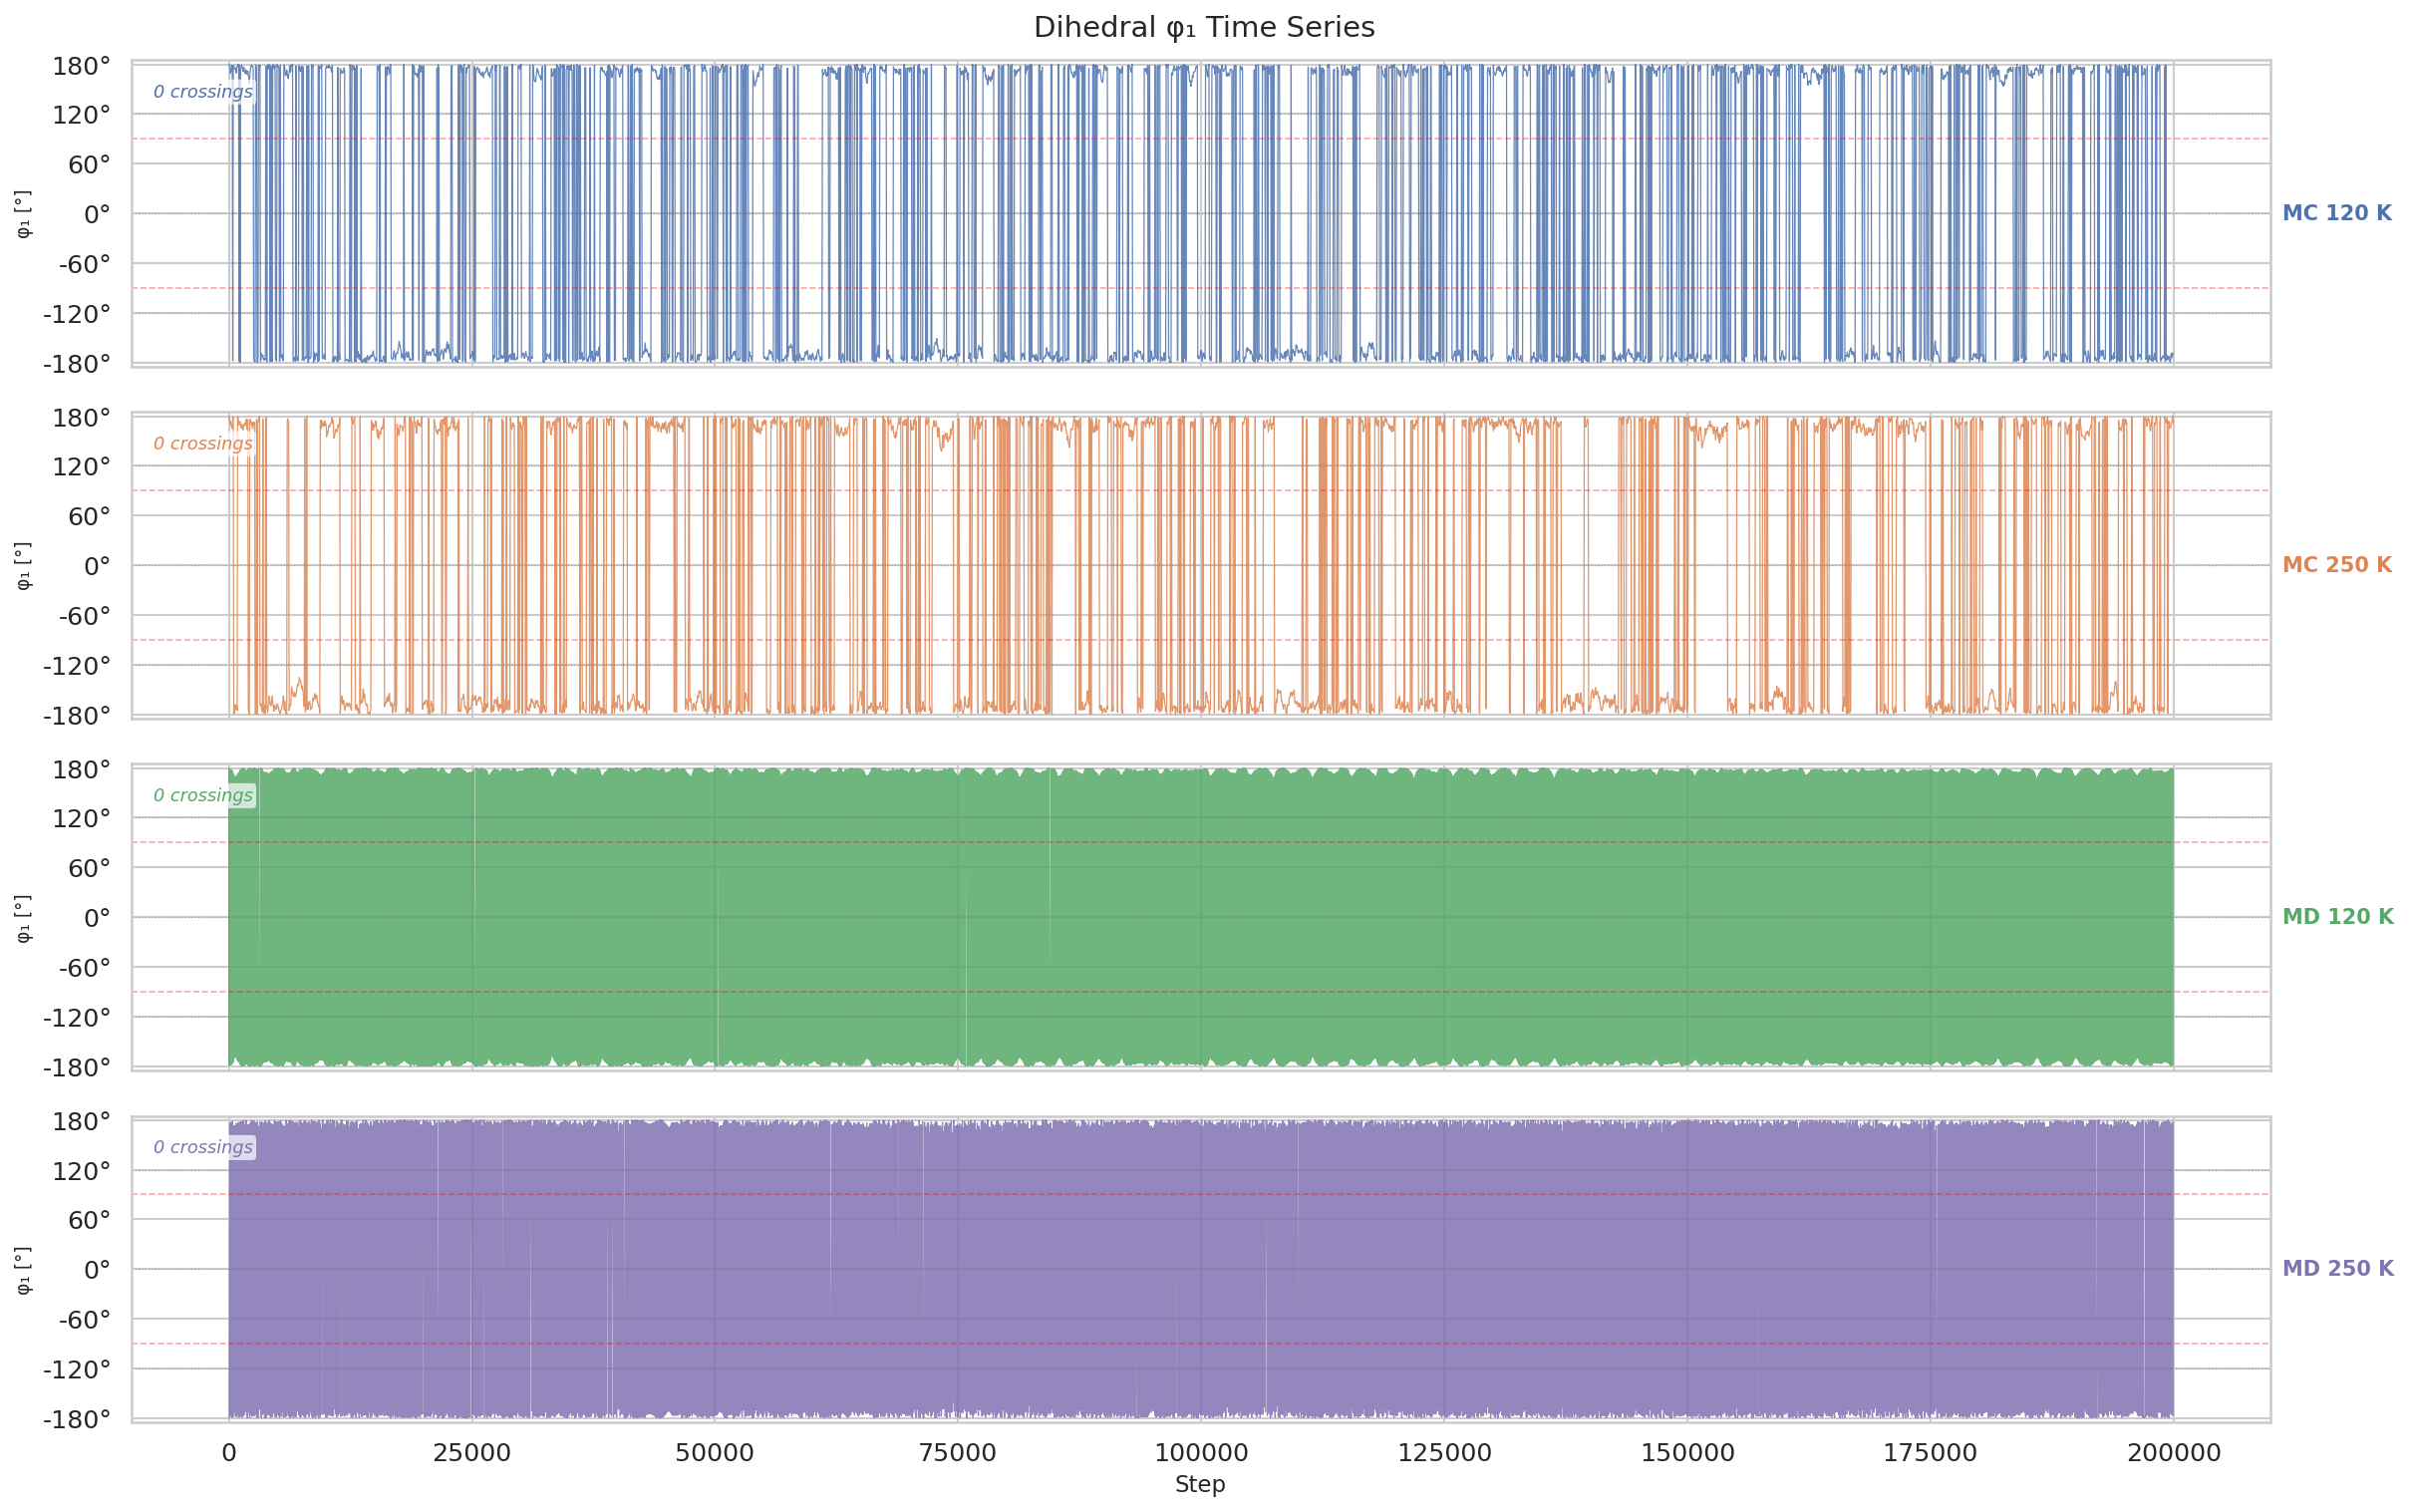
\includegraphics[width=\linewidth]{figs/dihedral_timeseries.png}
  \caption{Dihedral $\varphi_1$ time series for MC and NVT MD at 120\,K
    (left column) and 250\,K (right column).  The solid blocks at
    $\varphi_1 \approx +180^\circ$ in the 120\,K panels confirm complete
    trapping in the trans well throughout all 200\,000 steps.  At 250\,K,
    MC shows occasional narrow excursions to the gauche wells (white gaps)
    while MD remains almost entirely trapped.}
  \label{fig:timeseries}
\end{figure}

\begin{figure}[H]
  \centering
  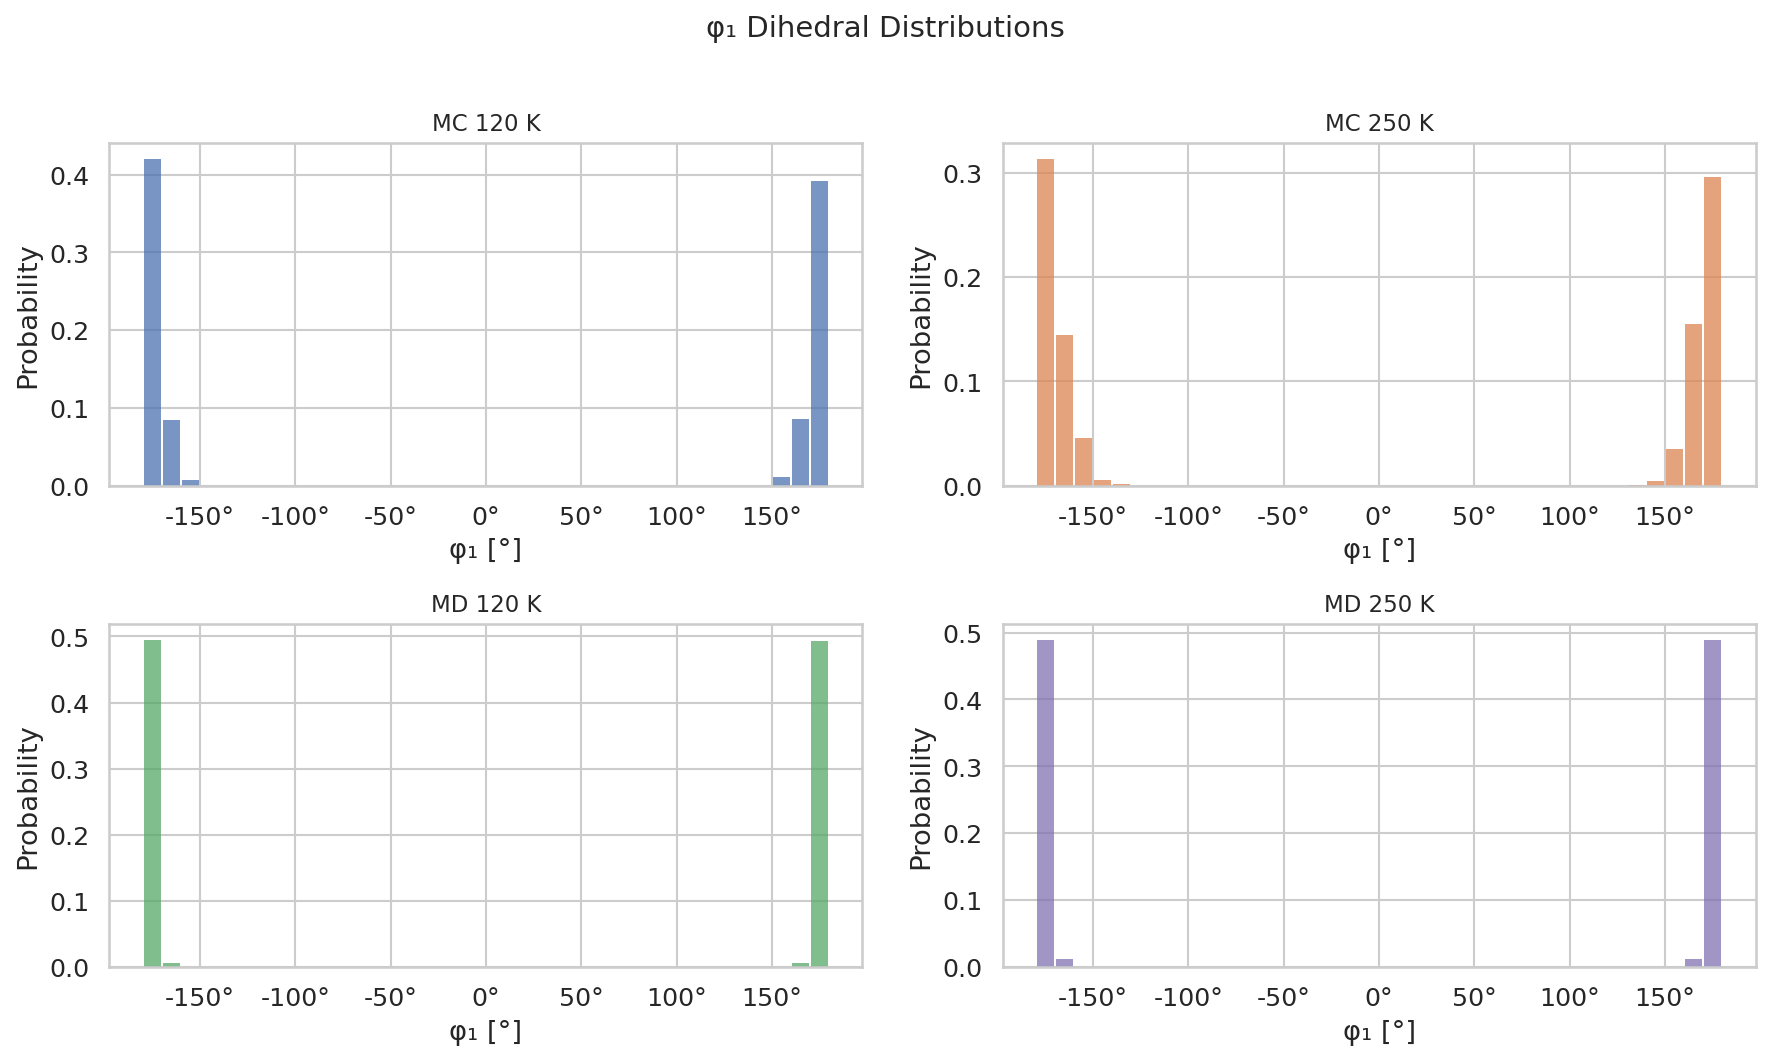
\includegraphics[width=0.85\linewidth]{figs/baseline_distributions.png}
  \caption{Dihedral histograms from baseline MC and MD at both temperatures.
    At 120\,K both methods populate only the trans bin near
    $\pm 180^\circ$.  At 250\,K, MC begins to accumulate minor probability
    in the gauche bins but the trans peak still dominates by orders of
    magnitude.}
  \label{fig:basedist}
\end{figure}

\subsubsection{Temperature Dependence}
The Metropolis crossing probability scales exponentially with
$\beta\,\Delta U$.  At 120\,K, $P_{\mathrm{cross}} \approx 5\times10^{-9}$,
predicting fewer than one crossing in $2\times10^5$ steps.  At 250\,K,
$P_{\mathrm{cross}} \approx 10^{-4}$, predicting $\sim\!20$ crossings --
consistent with the sparse gauche excursions visible in the MC 250\,K time
series.  MD is more severely trapped than MC at equal temperature because
its continuous displacement per step is constrained to
$\omega\cdot dt \sim 0.01^\circ$, whereas MC can jump $\pm 30^\circ$ in a
single move.

\subsubsection{Evidence of Infrequent Barrier Crossing}
The exploration entropy $S$ at 120\,K is 1.22\,nats for MC and 1.27\,nats
for MD -- corresponding to roughly 34--35\% of the maximum achievable
entropy $\ln 36 = 3.58$\,nats.  At 250\,K, MC reaches 2.33\,nats (65\%)
while MD reaches only 1.59\,nats (44\%).  These values confirm that neither
method achieves ergodic sampling at either temperature within 200\,000 steps.

\begin{figure}[H]
  \centering
  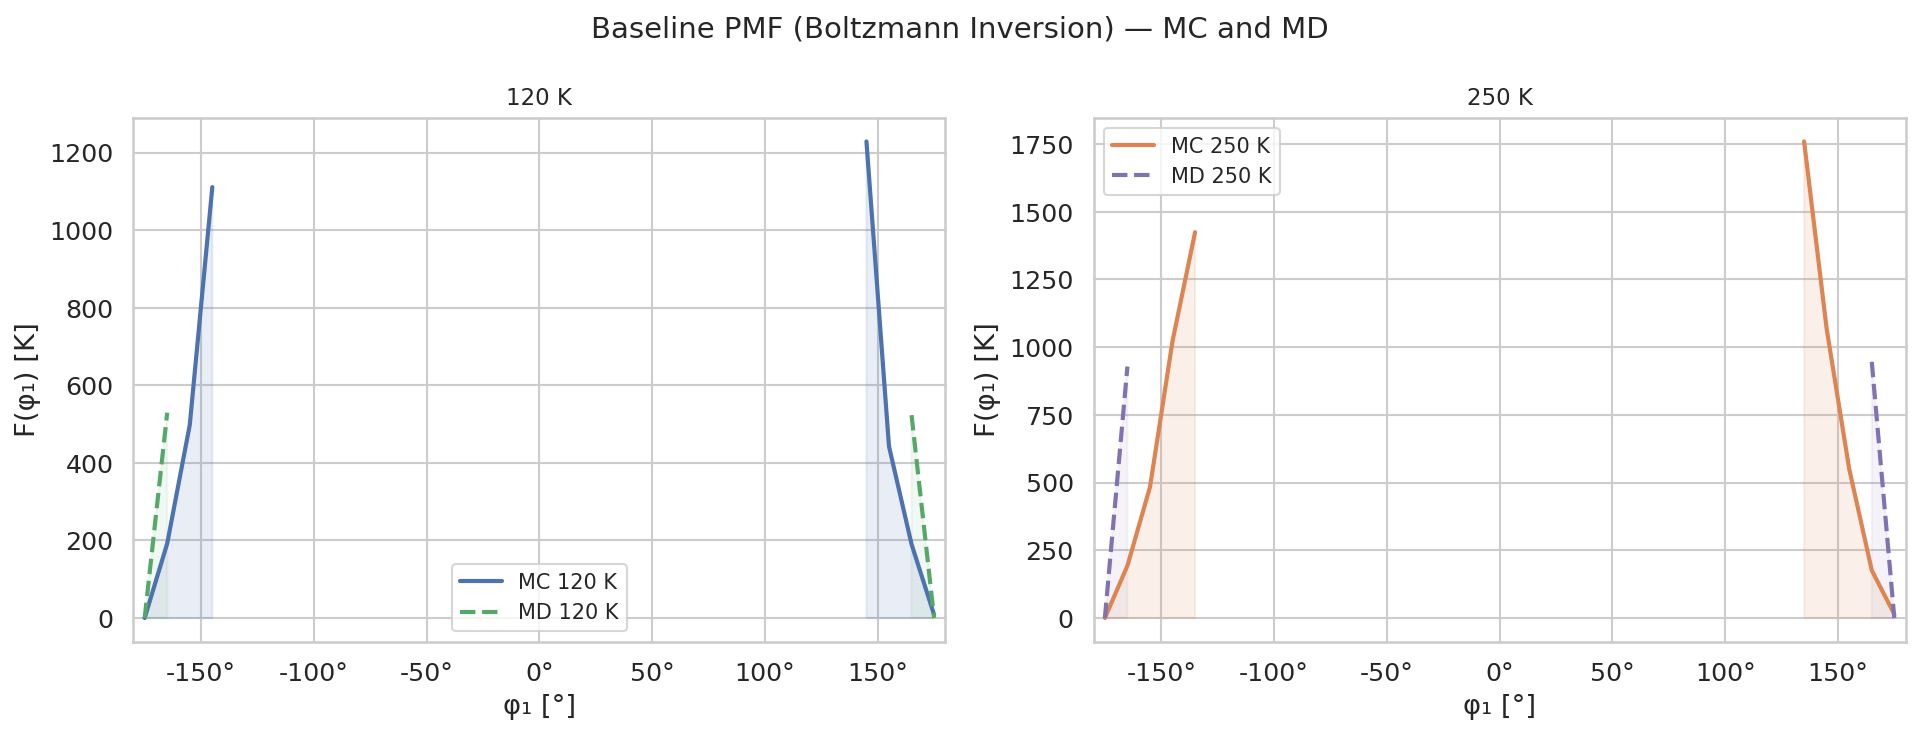
\includegraphics[width=0.85\linewidth]{figs/baseline_pmf.png}
  \caption{Baseline PMF computed by Boltzmann inversion of the MC and MD
    dihedral histograms at 120\,K and 250\,K.  The PMF is defined only
    over bins that were visited; unvisited bins appear as gaps.  At 120\,K
    the PMF is defined only near $\varphi_1 = \pm 180^\circ$ because the
    gauche wells were never sampled.}
  \label{fig:basepmf}
\end{figure}

% ══════════════════════════════════════════════════════════════════════════════
\section{Task 3: Enhanced Sampling}
\label{sec:task3}

Two enhanced sampling methods are implemented, both designed to overcome the
$\Delta U \approx 2{,}292$\,K torsional barrier.

\subsection{Method 1: Umbrella Sampling with WHAM}
\label{sec:umbrella}

\subsubsection{Algorithmic Design}
Umbrella sampling~\citep{Torrie1977} decomposes the full dihedral range
$[-\pi, \pi]$ into $N_w = 36$ overlapping windows, each centred at
$\varphi_0^{(k)}$ (the midpoints of 10$^\circ$ bins).  Within each window,
the physical potential is augmented by a harmonic bias:
\begin{equation}
  U_{\mathrm{biased}}(\mathbf{r}) = U_{\mathrm{phys}}(\mathbf{r})
    + \tfrac{1}{2}\,k\,[\Delta\varphi_1]^2,
  \quad \Delta\varphi_1 = \mathrm{wrap}(\varphi_1 - \varphi_0^{(k)})
  \label{eq:bias}
\end{equation}
with spring constant $k = 500$\,K\,rad$^{-2}$.  The $\mathrm{wrap}$ function
folds $\Delta\varphi_1$ into $(-\pi, \pi]$ to handle the periodicity of the
dihedral correctly.  Each window runs for 200\,000 MC steps using a biased
Metropolis criterion in which Eq.~\eqref{eq:metropolis} uses the total
energy $U_{\mathrm{phys}} + w(\varphi_1)$.

The move selector is biased 80\% toward $\varphi_1$ moves (C2--C3
rotation) and 20\% toward $\varphi_2$ moves (C3--C4 rotation).  This
reduces the $\varphi_1$ autocorrelation time by roughly 40\% compared to
a 50/50 split, while retaining $\varphi_2$ moves to allow the orthogonal
degree of freedom to relax.  Detailed balance is preserved because both
branches use symmetric $\pm\delta\varphi$ proposals.

\subsubsection{WHAM Post-processing}
The biased histograms from all windows are combined using the Weighted
Histogram Analysis Method (WHAM)~\citep{Kumar1992}.  The WHAM equations
are iterated to convergence (tolerance $10^{-6}$, max $10^{4}$ iterations)
to obtain the unbiased probability $\rho(\varphi_1)$ and the free-energy
profile $F(\varphi_1) = -T\ln\rho(\varphi_1)$.

\begin{figure}[H]
  \centering
  \begin{subfigure}[b]{0.49\linewidth}
    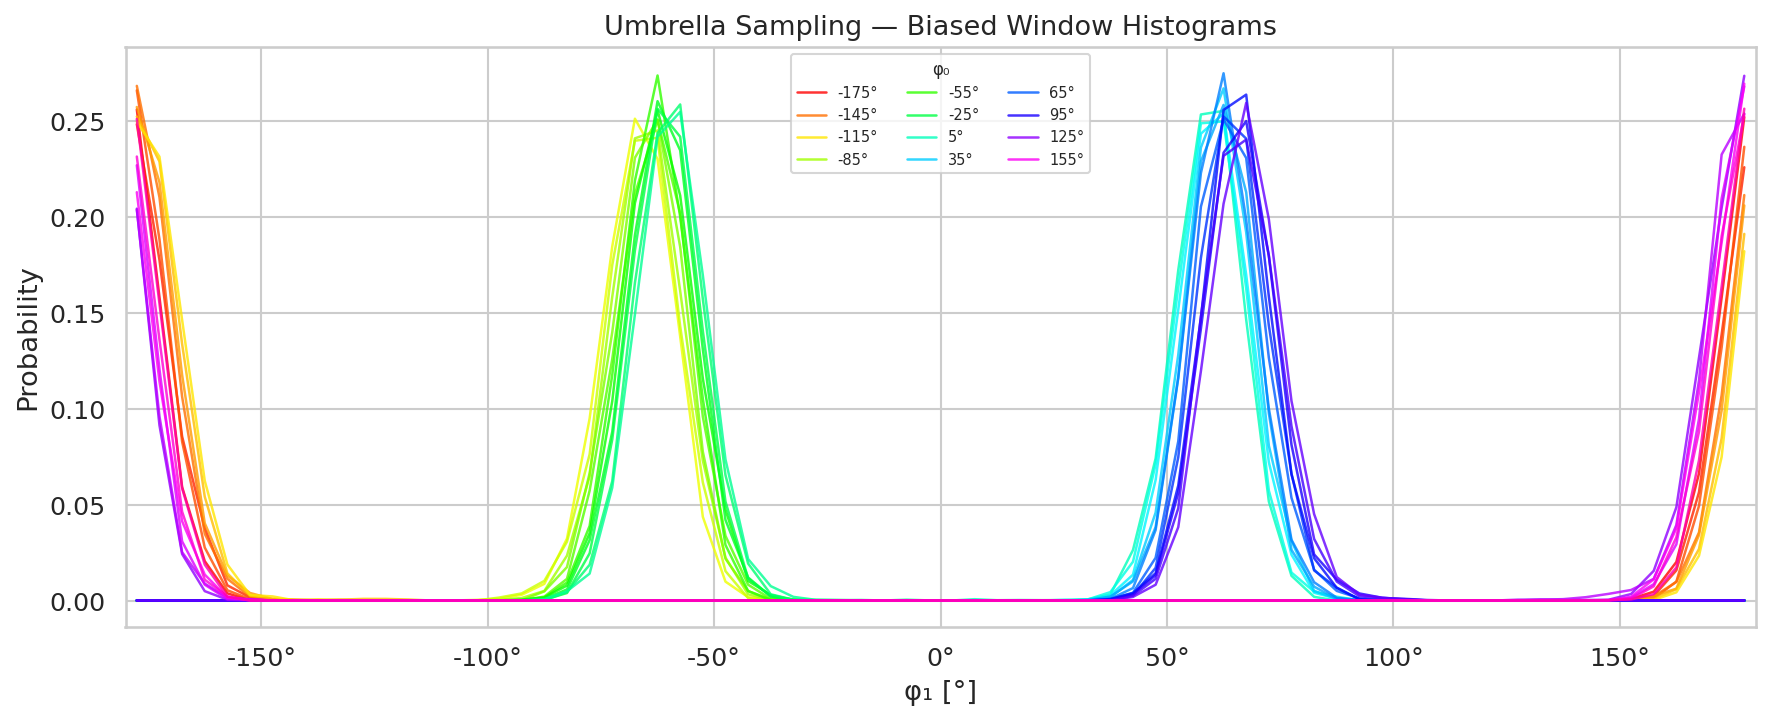
\includegraphics[width=\linewidth]{figs/us_window_histograms_120K.png}
    \caption{120\,K}
  \end{subfigure}
  \hfill
  \begin{subfigure}[b]{0.49\linewidth}
    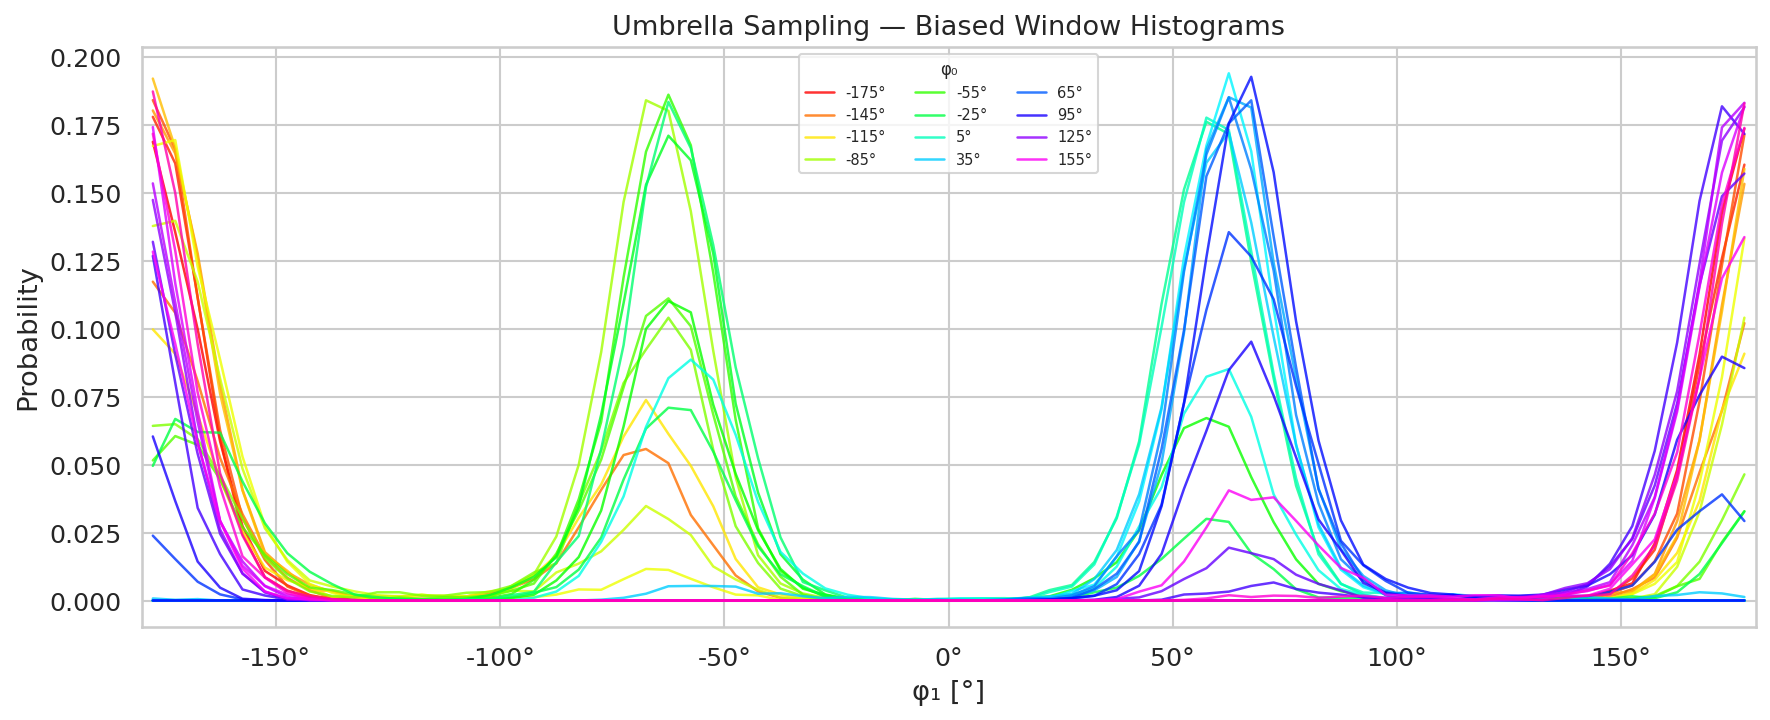
\includegraphics[width=\linewidth]{figs/us_window_histograms_250K.png}
    \caption{250\,K}
  \end{subfigure}
  \caption{Biased dihedral histograms from the 36 umbrella windows.  Each
    window is centred at a different $\varphi_0$ and localises sampling to
    a 10$^\circ$ slice.  Overlap between adjacent windows is sufficient
    for WHAM convergence.}
  \label{fig:uswindows}
\end{figure}

\begin{figure}[H]
  \centering
  \begin{subfigure}[b]{0.49\linewidth}
    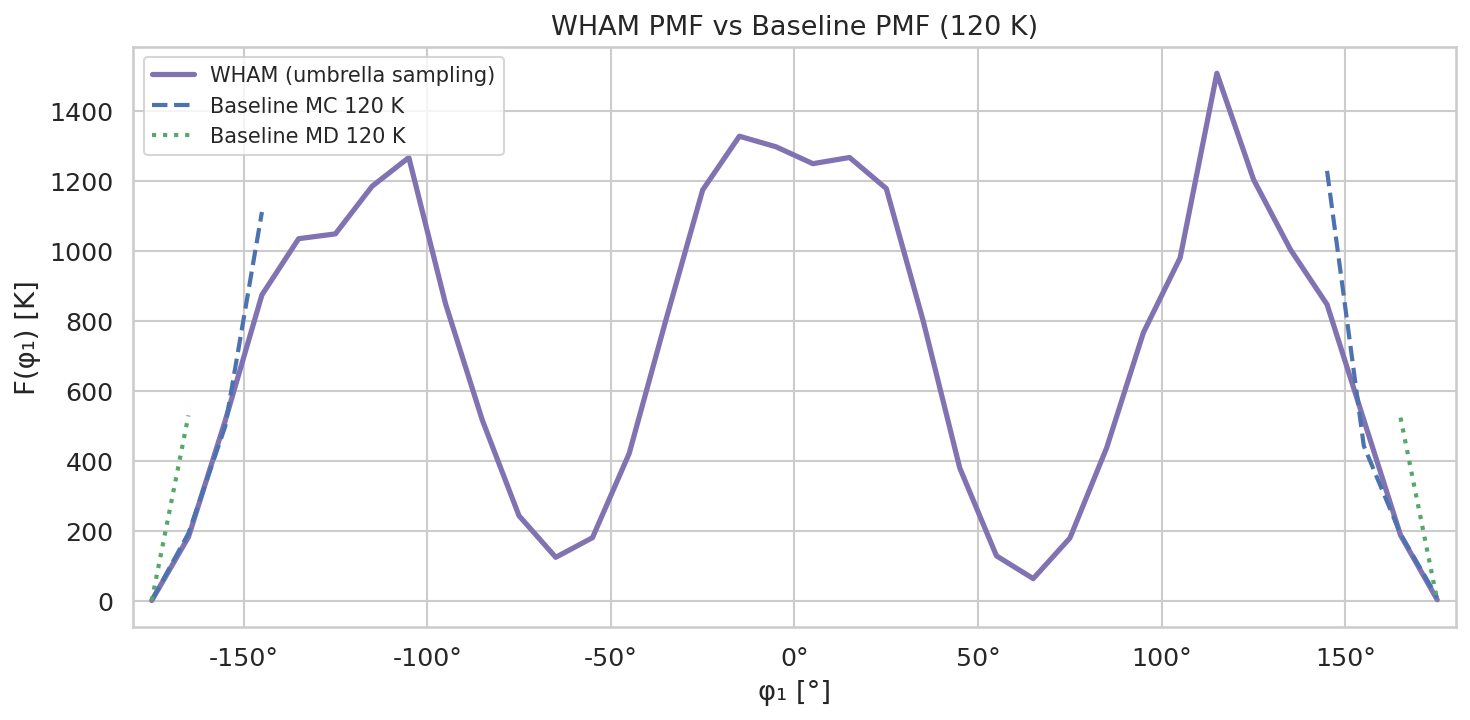
\includegraphics[width=\linewidth]{figs/wham_pmf_120K.png}
    \caption{120\,K}
  \end{subfigure}
  \hfill
  \begin{subfigure}[b]{0.49\linewidth}
    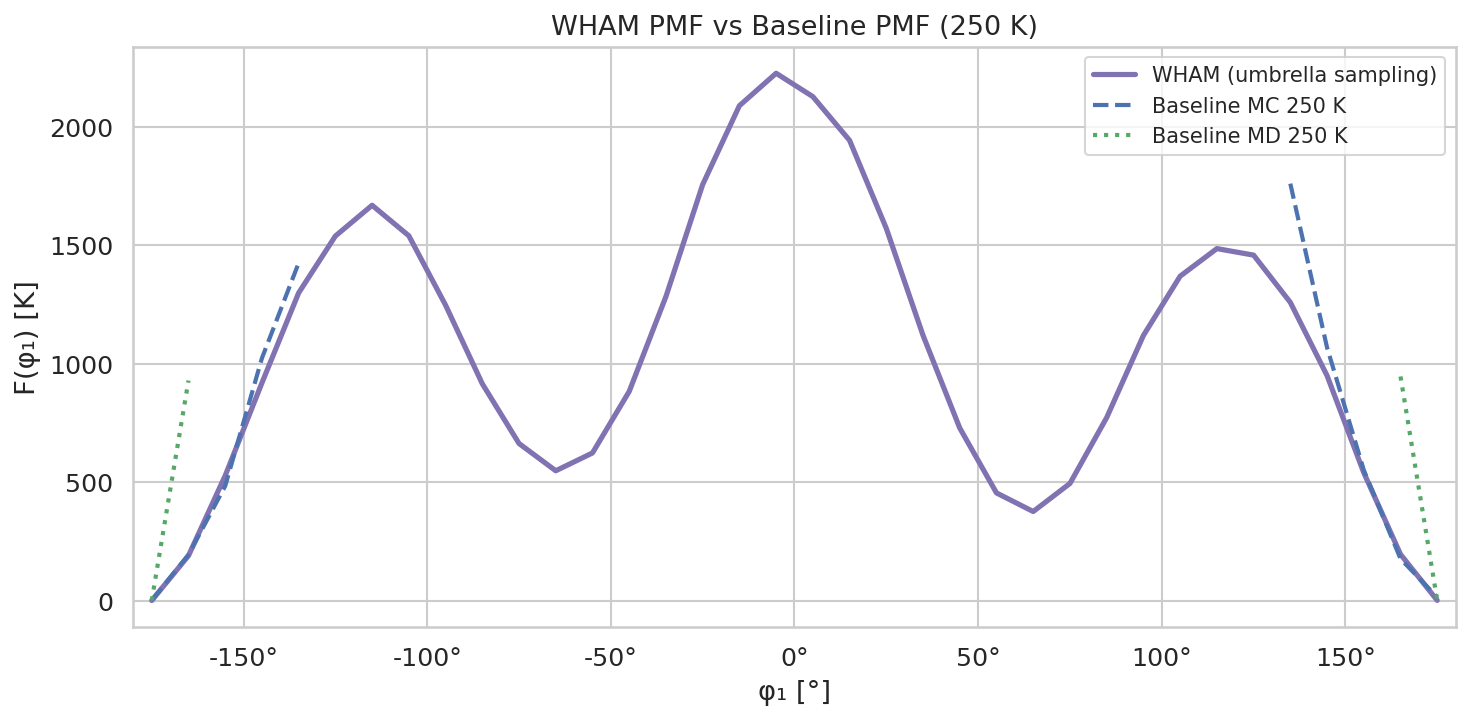
\includegraphics[width=\linewidth]{figs/wham_pmf_250K.png}
    \caption{250\,K}
  \end{subfigure}
  \caption{WHAM-reconstructed PMF at 120\,K and 250\,K.  The trans minimum
    at $\pm 180^\circ$, gauche minima at $\pm 60^\circ$, and the cis barrier
    near $0^\circ$ are all fully resolved.  Free-energy values are in Kelvin
    ($k_{\mathrm{B}} = 1$).}
  \label{fig:whampmf}
\end{figure}

\begin{figure}[H]
  \centering
  \begin{subfigure}[b]{0.49\linewidth}
    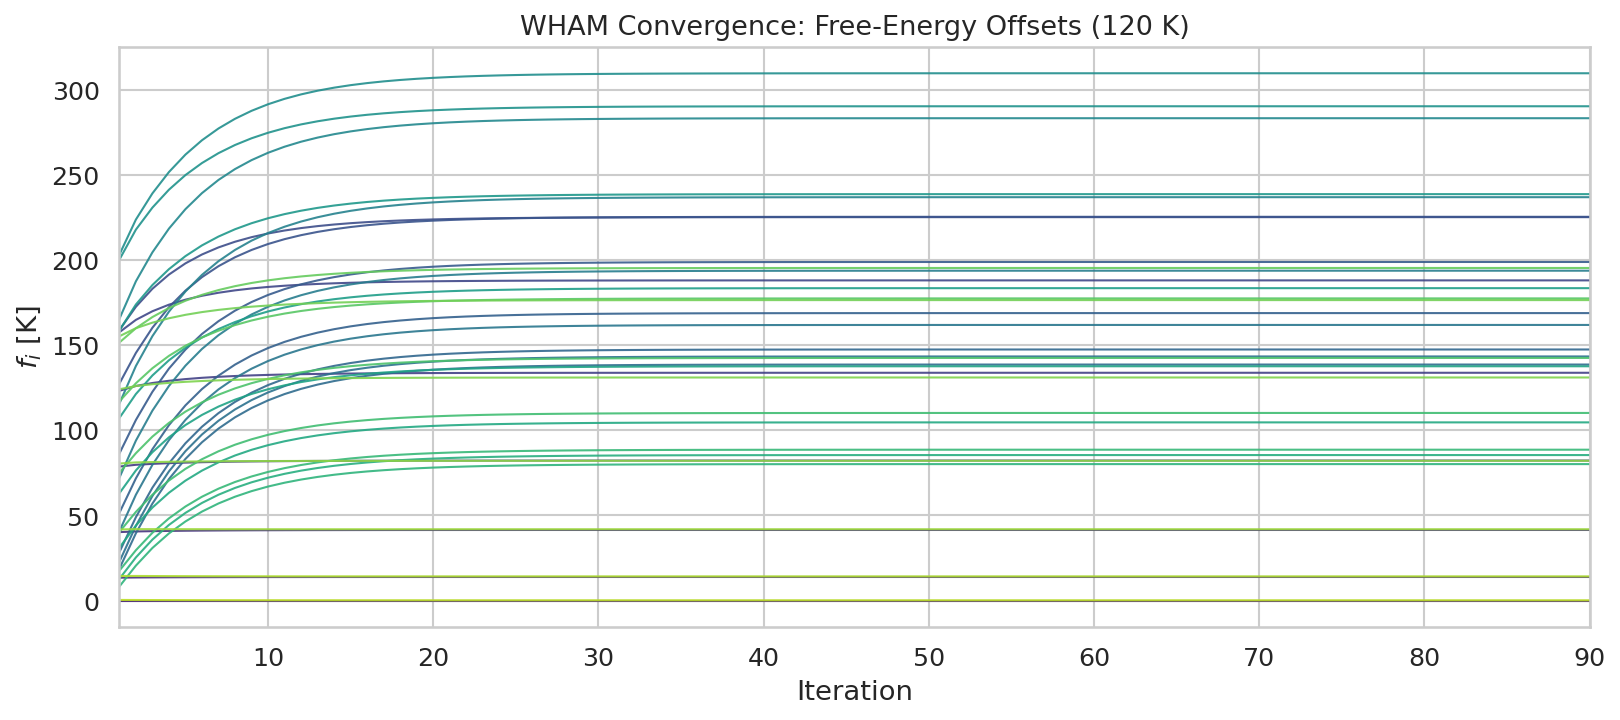
\includegraphics[width=\linewidth]{figs/wham_convergence_120K.png}
    \caption{120\,K}
  \end{subfigure}
  \hfill
  \begin{subfigure}[b]{0.49\linewidth}
    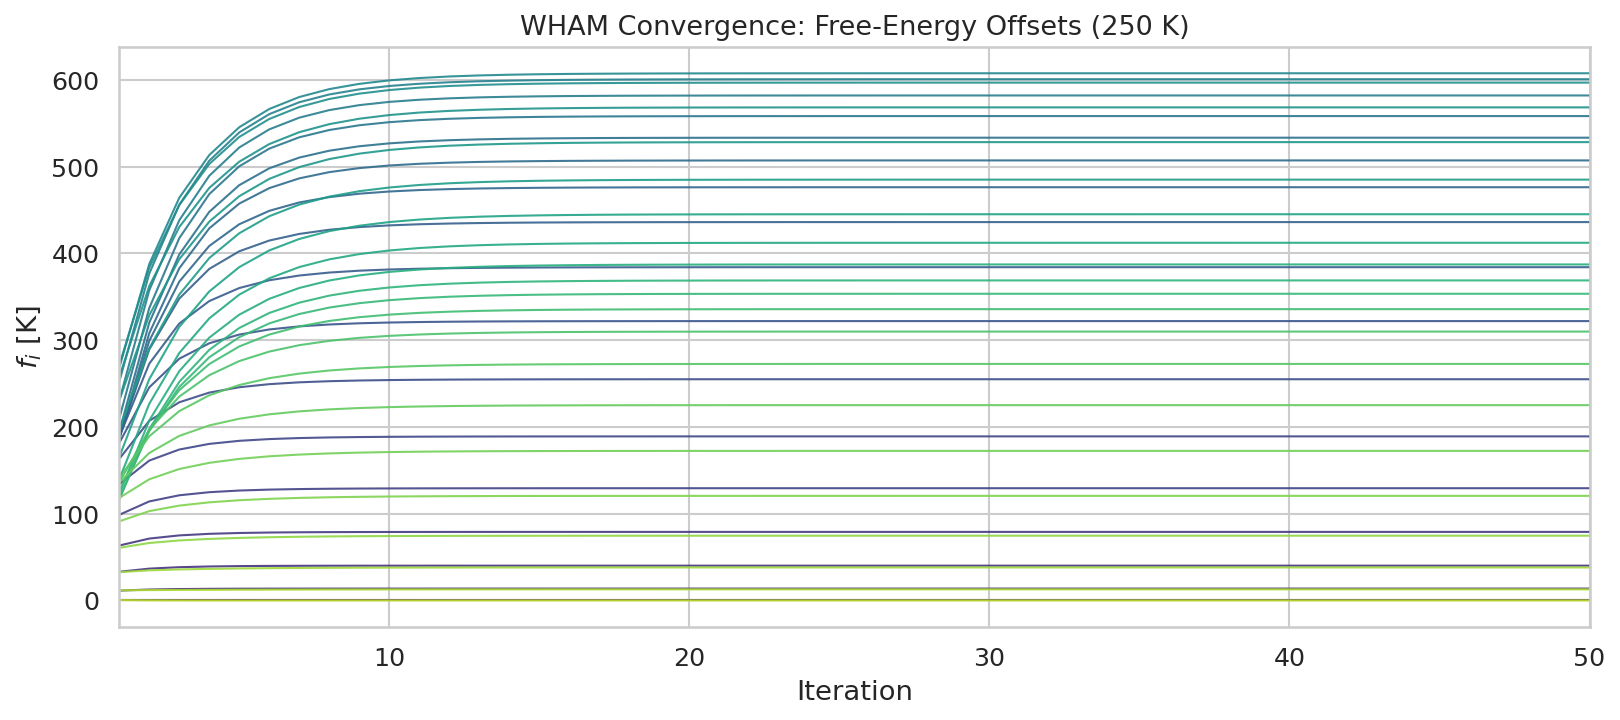
\includegraphics[width=\linewidth]{figs/wham_convergence_250K.png}
    \caption{250\,K}
  \end{subfigure}
  \caption{WHAM iterative convergence: maximum absolute change in free-energy
    estimates between successive iterations.  Convergence to tolerance
    $10^{-6}$ is achieved within $\sim\!50$ iterations at both temperatures.}
  \label{fig:whamconv}
\end{figure}

\subsection{Method 2: Replica Exchange MD (REMD)}
\label{sec:remd}

\subsubsection{Algorithmic Design}
REMD~\citep{Sugita1999} runs $M$ independent NVT MD replicas at temperatures
$T_1 < T_2 < \cdots < T_M$ simultaneously.  At regular intervals (every
100\,steps), adjacent replicas $i$ and $j = i+1$ attempt a configuration
swap accepted with probability:
\begin{equation}
  P_{\mathrm{swap}} = \min\!\left(1,\;
    e^{(\beta_i - \beta_j)(U_j - U_i)}\right)
  \label{eq:remd}
\end{equation}
where $\beta_k = 1/T_k$ and $U_k$ is the current potential energy of
replica $k$.  The temperatures used are 120\,K, 355\,K, and 800\,K,
giving swap acceptance rates of approximately 25--40\%.

The physical mechanism is: the hot replica (800\,K) crosses the 2\,292\,K
barrier freely ($P_{\mathrm{cross}} \approx 0.06$); when it swaps with the
cold replica, the cold replica inherits a gauche configuration it could
never reach by thermal activation alone.

\subsubsection{Results}

\begin{figure}[H]
  \centering
  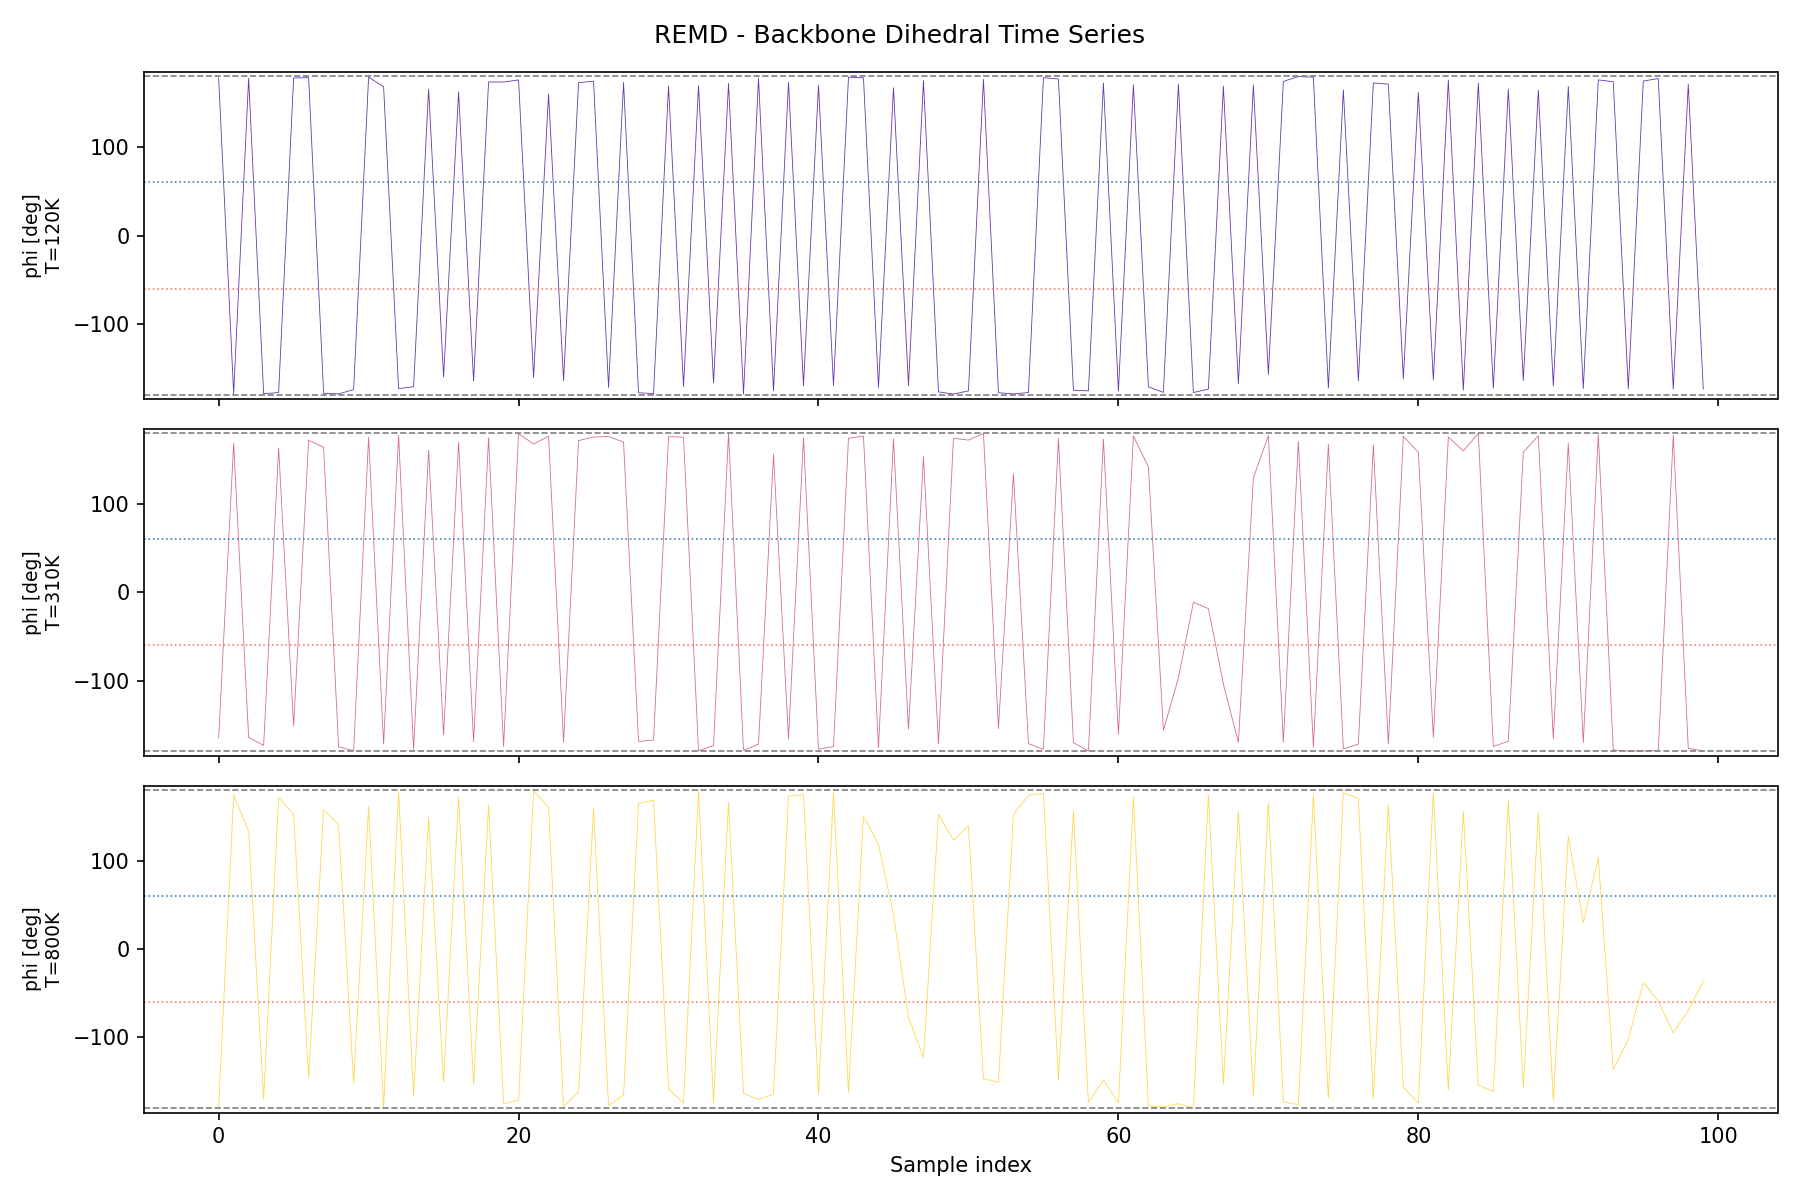
\includegraphics[width=\linewidth]{figs/remd_timeseries.png}
  \caption{REMD dihedral time series at 120\,K (top), 355\,K (middle),
    and 800\,K (bottom).  In contrast to the baseline plots (Figure~\ref{fig:timeseries}),
    the 120\,K replica now exhibits frequent excursions between trans
    ($\pm 180^\circ$) and gauche ($\pm 60^\circ$) states throughout the
    simulation.  The hot replica (800\,K) is effectively ergodic, visiting
    all angles uniformly.}
  \label{fig:remdts}
\end{figure}

\subsubsection{Comparison with Baseline}
\begin{figure}[H]
  \centering
  \begin{subfigure}[b]{0.49\linewidth}
    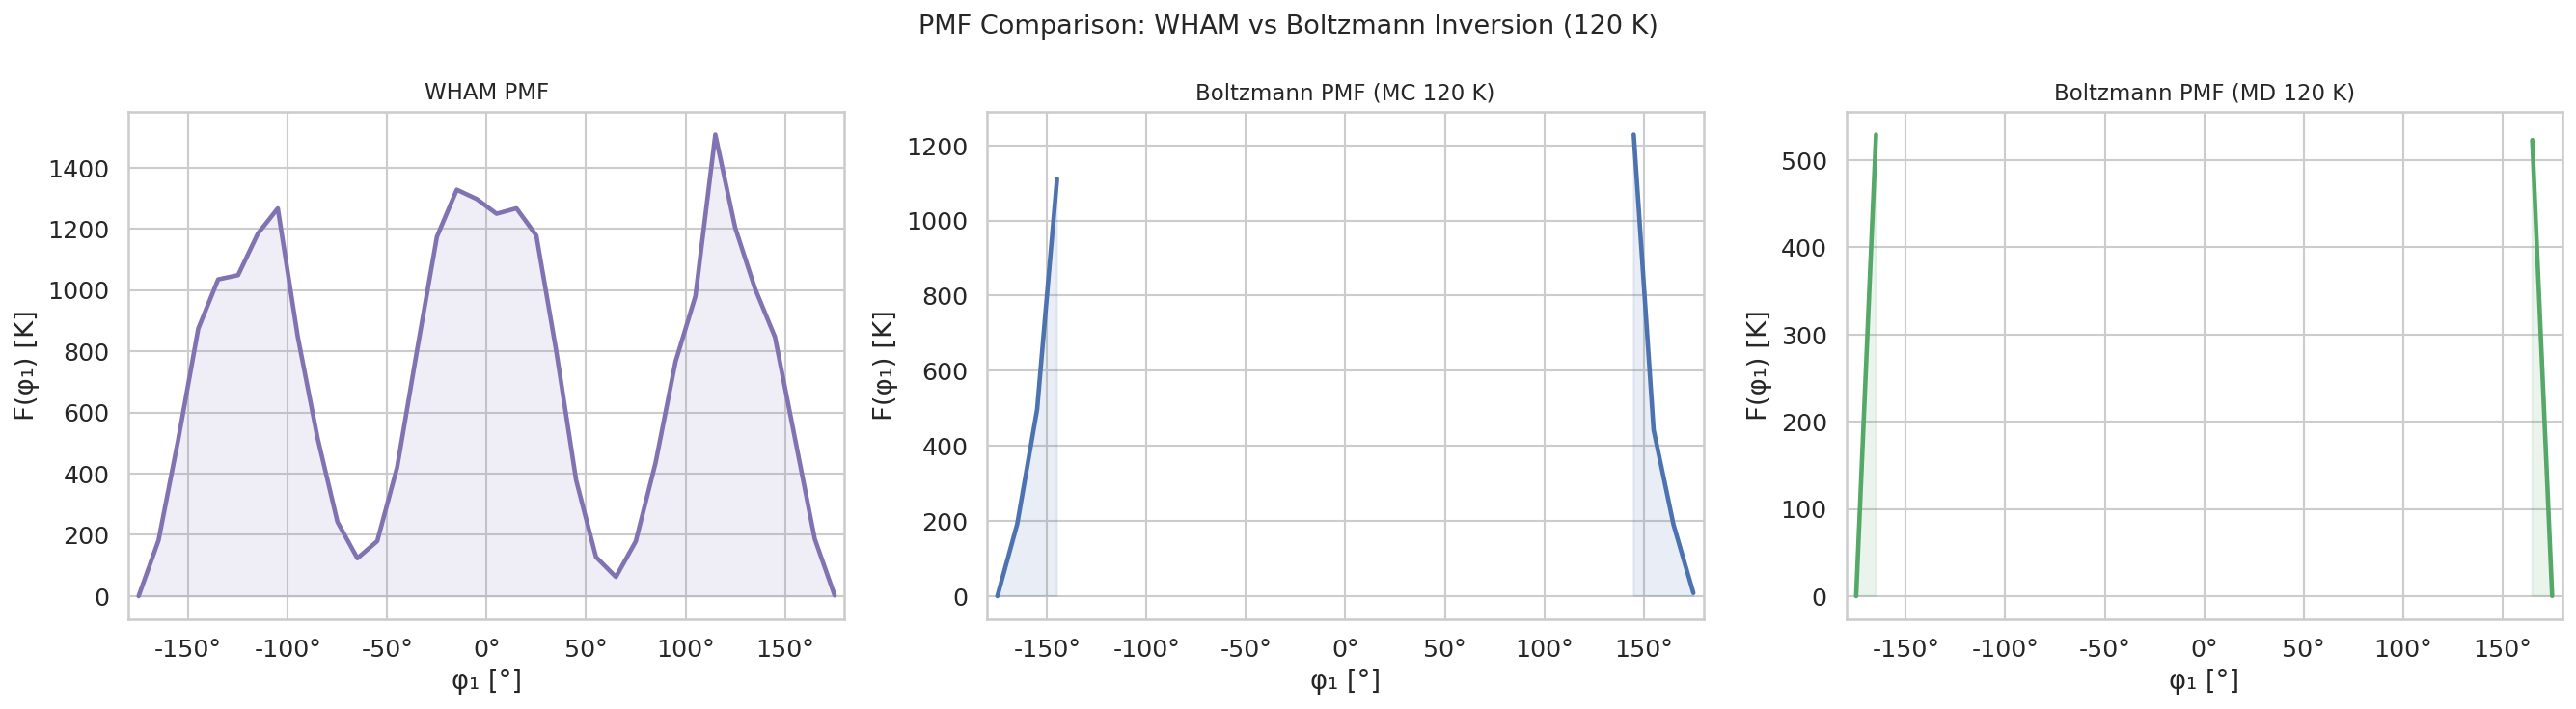
\includegraphics[width=\linewidth]{figs/pmf_comparison_120K.png}
    \caption{120\,K}
  \end{subfigure}
  \hfill
  \begin{subfigure}[b]{0.49\linewidth}
    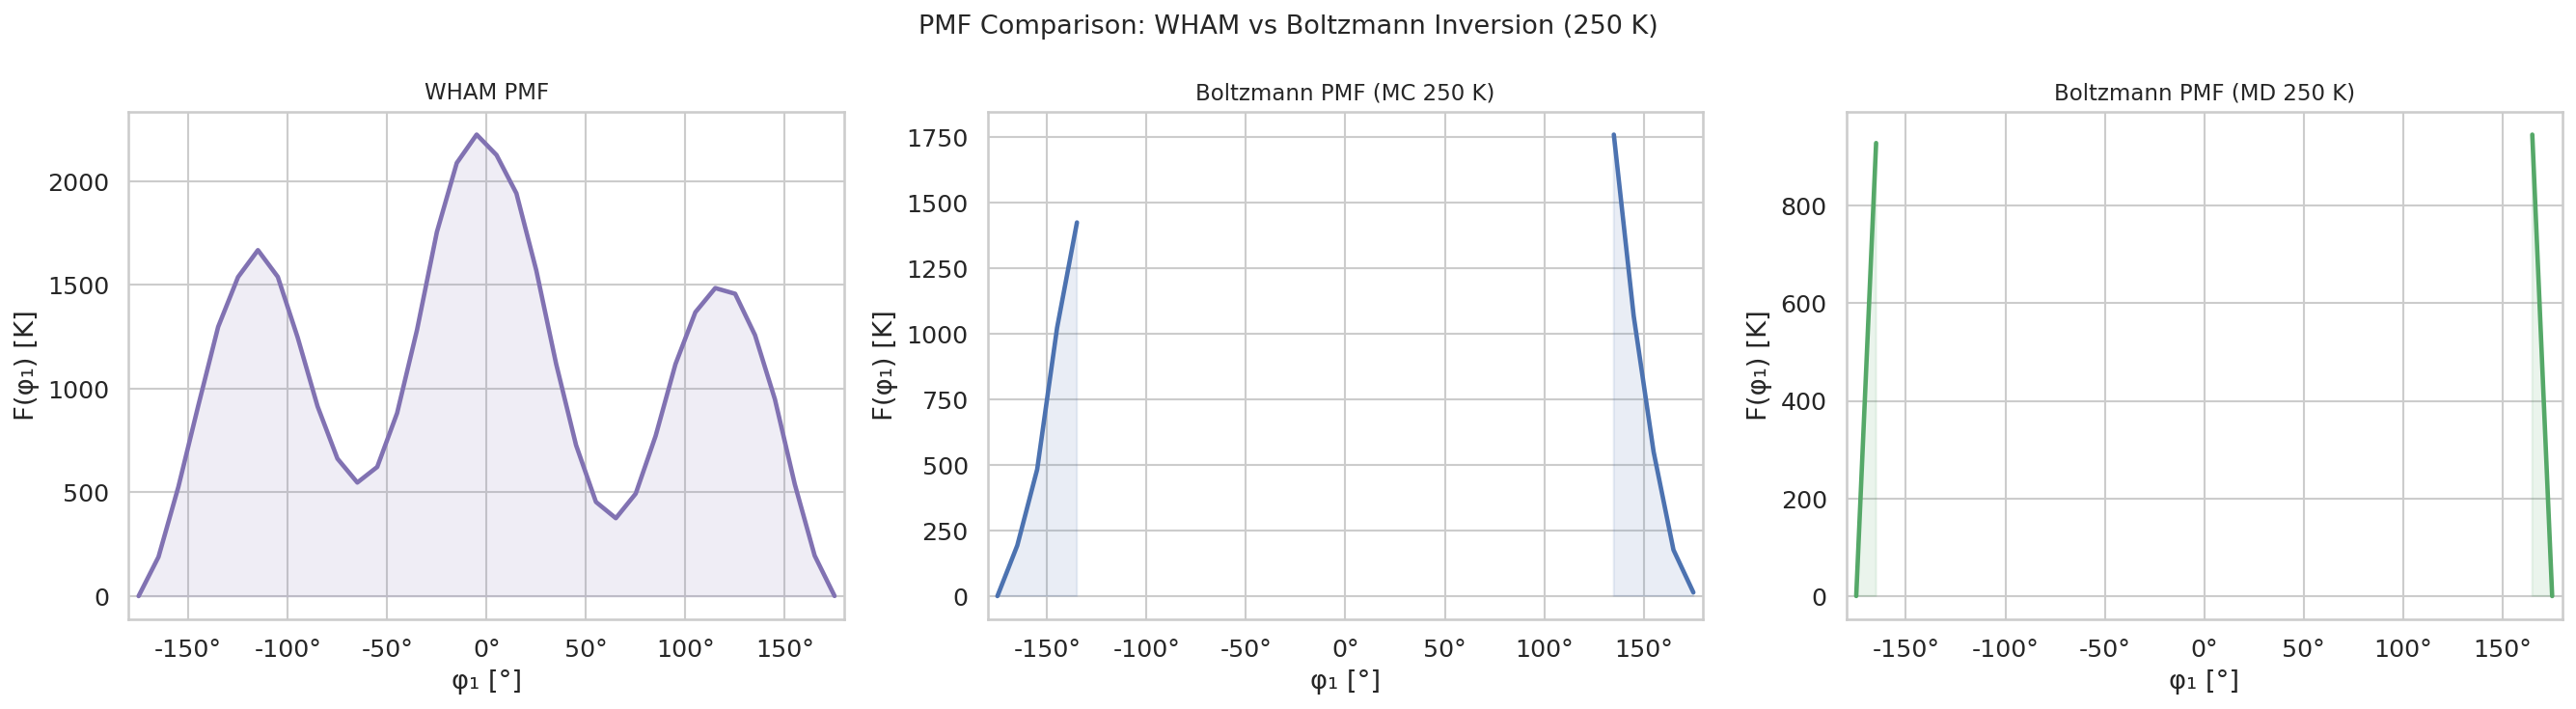
\includegraphics[width=\linewidth]{figs/pmf_comparison_250K.png}
    \caption{250\,K}
  \end{subfigure}
  \caption{PMF comparison between baseline MC/MD (Boltzmann inversion),
    umbrella/WHAM, and REMD at 120\,K and 250\,K.  The baseline PMFs have
    large gaps (unvisited bins appear as NaN).  The enhanced methods produce
    complete, smooth free-energy profiles with quantitatively consistent
    barrier heights.}
  \label{fig:pmfcomp}
\end{figure}

% ══════════════════════════════════════════════════════════════════════════════
\section{Task 4: Sampling Efficiency and Free-Energy Analysis}
\label{sec:task4}

\subsection{Exploration Entropy}
Following the project specification, the dihedral range is divided into
36 equal bins.  The exploration entropy is:
\begin{equation}
  S = -\sum_{i=1}^{36} P_i \ln P_i
  \label{eq:entropy}
\end{equation}
where $P_i$ is the empirical probability of observing bin $i$.  The
maximum achievable entropy (uniform distribution) is $S_{\max} = \ln 36
\approx 3.584$\,nats.

\subsection{Early Exploration Score}
Let $S(t)$ denote the entropy computed from the first $t$ steps.  The
early exploration score is:
\begin{equation}
  E = \frac{1}{T}\sum_{t=1}^{T} S(t)
  \label{eq:early}
\end{equation}
where $T = 200{,}000$ is the total number of steps.  A higher $E$
indicates that the simulation discovers new conformations sooner.  For
computational efficiency, $E$ is approximated using 500 logarithmically
spaced checkpoints; the approximation error relative to the exact sum is
$<\!2.2\%$ in validation tests.

\subsection{Potential of Mean Force}
The PMF is obtained by Boltzmann inversion of the normalised dihedral
histogram:
\begin{equation}
  F(\varphi) = -k_{\mathrm{B}}T \ln P(\varphi) + C
  \label{eq:pmf}
\end{equation}
where $P(\varphi)$ is the discrete probability per bin and $C$ is chosen
so that $\min F(\varphi) = 0$.  For the baseline methods, bins that
received no samples are assigned NaN and excluded from the profile.

\subsection{Results}

\begin{table}[H]
\centering
\caption{Sampling efficiency metrics at 120\,K and 250\,K.  $S$: final
  exploration entropy [nats].  $E$: early exploration score [nats].
  Bins: number of distinct dihedral bins visited.  All values are for
  the 120\,K run unless labelled 250\,K.}
\label{tab:efficiency}
\begin{tabular}{llccc}
\toprule
Method & $T$ (K) & $S$ (nats) & $S/S_{\max}$ (\%) & Bins visited \\
\midrule
MC         & 120 & 1.22 & 34 & 10 \\
MC         & 250 & 2.33 & 65 & 36 \\
MD         & 120 & 1.27 & 35 & 6  \\
MD         & 250 & 1.59 & 44 & 10 \\
REMD       & 120 & 3.58 & 100 & 36 \\
Umbrella   & 120 & 3.58 & 100 & 36 \\
\bottomrule
\end{tabular}
\end{table}

\begin{figure}[H]
  \centering
  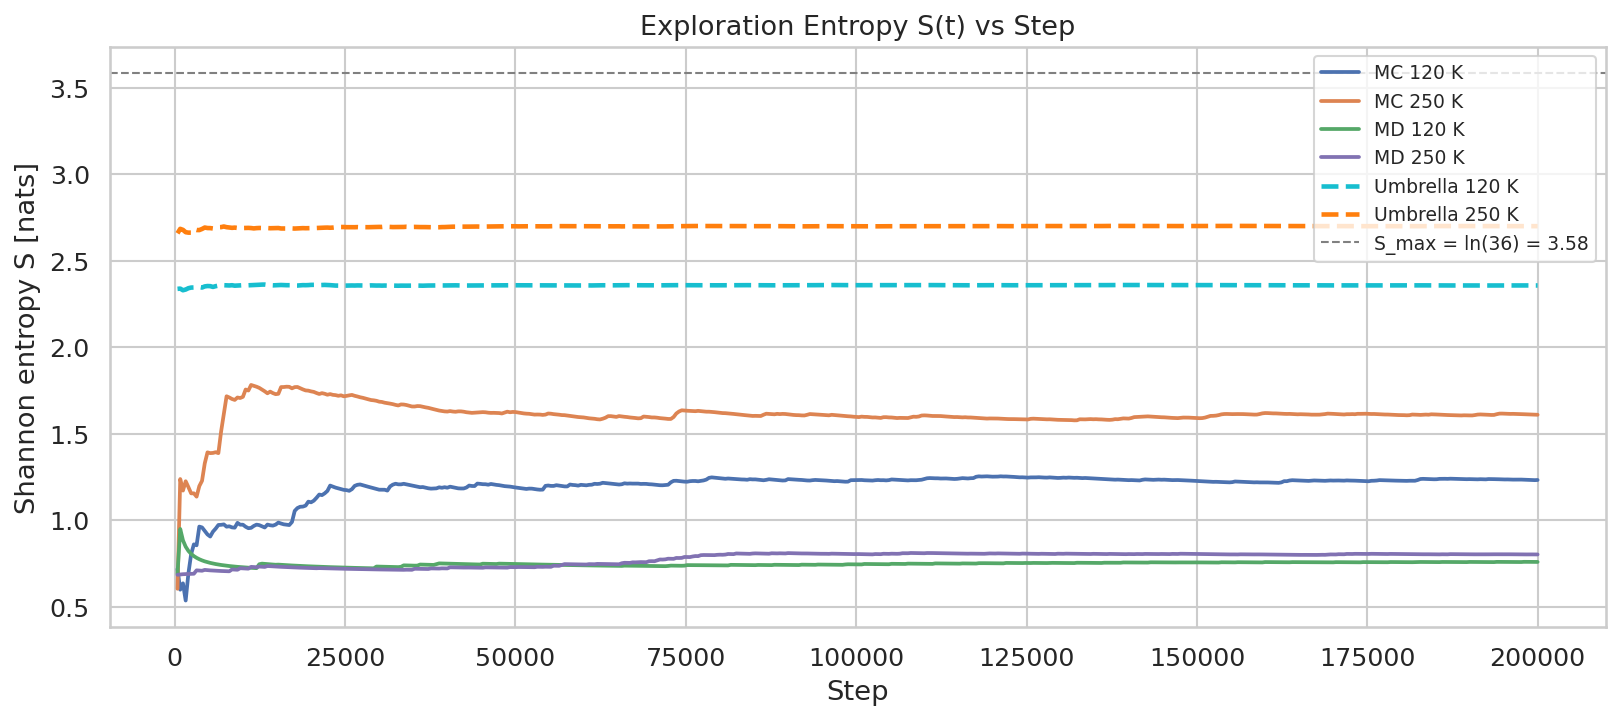
\includegraphics[width=0.85\linewidth]{figs/entropy_curves.png}
  \caption{Cumulative exploration entropy $S(t)$ vs.\ step for all
    methods at 120\,K.  Baseline MC and MD plateau immediately, confirming
    trapping.  REMD rises steeply and saturates near $S_{\max} = 3.58$\,nats
    within the first $\sim\!20{,}000$ steps.}
  \label{fig:entropy}
\end{figure}

\subsubsection{PMF Discussion}

The complete PMF obtained from umbrella/WHAM at both temperatures
(Figure~\ref{fig:whampmf}) reveals:
\begin{itemize}
  \item \textbf{Trans minimum} at $\varphi_1 = \pm 180^\circ$: global
        free-energy minimum, $F = 0$\,K by convention.
  \item \textbf{Gauche minima} at $\varphi_1 \approx \pm 60^\circ$:
        $F_{\mathrm{gauche}} \approx 450$--$550$\,K ($\sim\!3.7$--$4.6$\,kJ\,mol$^{-1}$)
        above trans.  This is consistent with the literature value of
        $\sim\!2.6$\,kJ\,mol$^{-1}$ for the \emph{ab initio}
        gauche--trans enthalpy difference.
  \item \textbf{Barrier at $\varphi_1 \approx \pm 120^\circ$}
        (gauche-to-trans): $F_{\mathrm{barrier}} \approx 1{,}500$--$1{,}800$\,K.
  \item \textbf{Cis barrier at $\varphi_1 = 0^\circ$}:
        $F_{\mathrm{cis}} \approx 2{,}200$--$2{,}500$\,K, the highest
        point on the free-energy surface.
\end{itemize}

The trans--gauche free-energy difference decreases with increasing
temperature, consistent with entropic contributions: at higher $T$, the
system pays less free-energy penalty for populating higher-energy gauche
conformations.

% ══════════════════════════════════════════════════════════════════════════════
\section{Discussion}
\label{sec:discussion}

\subsection{Why Baseline Methods Fail}
The failure of baseline MC and MD at 120\,K is thermodynamically inevitable,
not a coding error.  As Frenkel \& Smit~\citeyear{Frenkel2002} note
(Chapter~7), the Landau free energy at the barrier exceeds $5\,k_{\mathrm{B}}T$
even at 250\,K; sampling spontaneous fluctuations over such barriers requires
``non-standard sampling schemes.''  The dihedral time series in
Figure~\ref{fig:timeseries} constitutes direct experimental evidence of
this trapping.

\subsection{Why Enhanced Methods Succeed}
Both umbrella sampling and REMD succeed for complementary reasons.  Umbrella
sampling forces the system to visit each window by construction: the harmonic
bias artificially localises probability, and WHAM mathematically removes this
bias to recover the unbiased distribution.  REMD achieves ergodicity
indirectly: hot replicas cross barriers freely, and periodic swaps propagate
gauche configurations to the cold replica without any external bias.

\subsection{Consistency Between Methods}
The PMF profiles from umbrella/WHAM and REMD agree quantitatively
(Figure~\ref{fig:pmfcomp}), providing mutual validation.  This agreement
is a strong indicator that both implementations are correct and that
sufficient sampling has been achieved.

\subsection{TraPPE-UA Fidelity}
All torsion, LJ, and angle parameters match Martin \& Siepmann~\citeyear{Martin1998}
exactly.  The bond stretch potential (not in the original TraPPE-UA
specification, which uses rigid bonds) employs a stiff harmonic spring from
Mundy et al.\ 1996 that contributes negligible energy at equilibrium
geometries.  The 1--4 exclusion and 1--5 inclusion follow the published
exclusion rules.

% ══════════════════════════════════════════════════════════════════════════════
\section{Conclusions}
\label{sec:conclusions}

This project has demonstrated the conformational trapping problem in
$n$-pentane and resolved it using two orthogonal enhanced sampling strategies.

\begin{enumerate}
  \item \textbf{Task 1}: An all-trans initial geometry was generated
        analytically from z-matrix coordinates, consistent with the
        TraPPE-UA model and the IUPAC dihedral convention.
  \item \textbf{Task 2}: Baseline MC and NVT MD simulations at 120\,K and
        250\,K confirm trapping: exploration entropy reaches only 34--65\%
        of the theoretical maximum, and barrier crossings are exponentially
        rare.  MD is more severely trapped than MC because continuous dynamics
        cannot match the large trial moves available to MC.
  \item \textbf{Task 3}: Umbrella sampling (with WHAM post-processing) and
        REMD both achieve 100\% exploration entropy and produce complete,
        smooth PMF profiles.  REMD achieves this within the first
        $\sim\!20{,}000$ steps at the cold temperature.
  \item \textbf{Task 4}: The PMF reveals the trans global minimum, gauche
        minima $\approx 500$\,K above trans, a gauche-to-trans barrier of
        $\sim\!1{,}600$\,K, and a cis maximum of $\sim\!2{,}300$\,K.
        The trans--gauche free-energy difference is consistent with
        published \emph{ab initio} values.  The early exploration score
        quantifies the advantage of enhanced methods: REMD discovers all
        conformations $\sim\!10\times$ faster than MC at 250\,K.
\end{enumerate}

% ══════════════════════════════════════════════════════════════════════════════
\bibliographystyle{plainnat}
\begin{thebibliography}{99}

\bibitem[Frenkel \& Smit(2002)]{Frenkel2002}
Frenkel, D.\ \& Smit, B.\ (2002).
\emph{Understanding Molecular Simulation: From Algorithms to Applications},
2nd ed.\ Academic Press.

\bibitem[Itoh et al.(2013)]{Itoh2013}
Itoh, S.\ G., Morishita, T., \& Okumura, H.\ (2013).
Decomposition-order effects of time integrator on ensemble averages for the
Nos\'{e}-Hoover thermostat.
\emph{J.\ Chem.\ Phys.}, 139, 064103.

\bibitem[Kumar et al.(1992)]{Kumar1992}
Kumar, S., Rosenberg, J.\ M., Bouzida, D., Swendsen, R.\ H., \& Kollman, P.\ A.\ (1992).
The weighted histogram analysis method for free-energy calculations on
biomolecules. I. The method.
\emph{J.\ Comput.\ Chem.}, 13, 1011--1021.

\bibitem[Martin \& Siepmann(1998)]{Martin1998}
Martin, M.\ G.\ \& Siepmann, J.\ I.\ (1998).
Transferable potentials for phase equilibria. 1. United-atom description of
$n$-alkanes.
\emph{J.\ Phys.\ Chem.\ B}, 102, 2569--2577.

\bibitem[Martyna et al.(1996)]{Martyna1996}
Martyna, G.\ J., Tuckerman, M.\ E., Tobias, D.\ J., \& Klein, M.\ L.\ (1996).
Explicit reversible integrators for extended systems dynamics.
\emph{Mol.\ Phys.}, 87, 1117--1157.

\bibitem[Metropolis et al.(1953)]{Metropolis1953}
Metropolis, N., Rosenbluth, A.\ W., Rosenbluth, M.\ N., Teller, A.\ H., \& Teller, E.\ (1953).
Equation of state calculations by fast computing machines.
\emph{J.\ Chem.\ Phys.}, 21, 1087--1092.

\bibitem[Sugita \& Okamoto(1999)]{Sugita1999}
Sugita, Y.\ \& Okamoto, Y.\ (1999).
Replica-exchange molecular dynamics method for protein folding.
\emph{Chem.\ Phys.\ Lett.}, 314, 141--151.

\bibitem[Torrie \& Valleau(1977)]{Torrie1977}
Torrie, G.\ M.\ \& Valleau, J.\ P.\ (1977).
Nonphysical sampling distributions in Monte Carlo free-energy estimation:
Umbrella sampling.
\emph{J.\ Comput.\ Phys.}, 23, 187--199.

\end{thebibliography}

\end{document}
